\chapter{Boolean Logic}
\chaplabel{logic}

This introduces some basic Boolean logic including gates and Boolean algebra.

\begin{figure}[!htb]
	\centering
	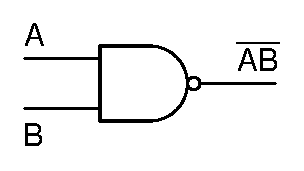
\includegraphics[scale=0.7]{logic/NAND.eps}
	\caption{The NAND gate outputs NOT(A AND B).}
	\label{fig:nand}
  \end{figure} 